\documentclass{beamer}
\usepackage[utf8]{inputenc}

\usetheme{Madrid}
\usecolortheme{default}
\usepackage{amsmath,amssymb,amsfonts,amsthm}
\usepackage{txfonts}
\usepackage{tkz-euclide}
\usepackage{listings}
\usepackage{adjustbox}
\usepackage{array}
\usepackage{tabularx}
\usepackage{gvv}
\usepackage{lmodern}
\usepackage{circuitikz}
\usepackage{tikz}
\usepackage{graphicx}

\setbeamertemplate{page number in head/foot}[totalframenumber]

\usepackage{tcolorbox}
\tcbuselibrary{minted,breakable,xparse,skins}

\definecolor{bg}{gray}{0.95}
\DeclareTCBListing{mintedbox}{O{}m!O{}}{%
  breakable=true,
  listing engine=minted,
  listing only,
  minted language=#2,
  minted style=default,
  minted options={%
    linenos,
    gobble=0,
    breaklines=true,
    fontsize=\small,
    numbersep=8pt,
    #1},
  boxsep=0pt,
  left=25pt,
  right=0pt,
  top=3pt,
  bottom=3pt,
  arc=5pt,
  leftrule=0pt,
  rightrule=0pt,
  bottomrule=2pt,
  toprule=2pt,
  colback=bg,
  colframe=orange!70,
  enhanced,
  overlay={%
    \begin{tcbclipinterior}
    \fill[orange!20!white] (frame.south west) rectangle ([xshift=20pt]frame.north west);
    \end{tcbclipinterior}},
}

%------------------------------------------------------------

\title{4.10.9}
\date{October 2025}
\author{Anshu Kumar Ram - EE25BTECH11009}

\begin{document}

\frame{\titlepage}

%------------------------------------------------------------
\begin{frame}{Question}
Find the equation of the plane passing through the line of intersection of the planes
\begin{align}
\vec{r} \cdot (\hat{i} + 2\hat{j} + 3\hat{k}) - 4 &= 0,\\
\vec{r} \cdot (2\hat{i} + \hat{j} - \hat{k}) + 5 &= 0
\end{align}
and which is perpendicular to the plane
\begin{align}
\vec{r} \cdot (5\hat{i} + 3\hat{j} - 6\hat{k}) + 8 &= 0.
\end{align}
\end{frame}

%------------------------------------------------------------
\begin{frame}{Solution - Step 1}
The required plane can be written as a linear combination of the first two planes
\begin{align}
(\vec{n}_1 + \lambda\vec{n}_2)^T\vec{r} = c_1 + \lambda c_2
\end{align}
where
\begin{align}
\vec{n}_1 = \myvec{1 \\ 2 \\ 3}, \quad c_1 = 4 \\
\vec{n}_2 = \myvec{2 \\ 1 \\ -1}, \quad c_2 = -5
\end{align}
and it is perpendicular to
\begin{align}
\vec{r}\cdot \myvec{5 \\ 3 \\ -6} + 8 = 0
\end{align}
\end{frame}

%------------------------------------------------------------
\begin{frame}{Solution - Step 2}
For perpendicular planes,
\begin{align}
\vec{n}^T \vec{n}_3 = 0, \quad \vec{n}_3 = \myvec{5 \\ 3 \\ -6}
\end{align}
Substituting,
\begin{align}
(\vec{n}_1 + \lambda\vec{n}_2)^T\vec{n}_3 = 0
\end{align}
\begin{align}
\myvec{1 & 2 & 3}\myvec{5 \\ 3 \\ -6} + \lambda\myvec{2 & 1 & -1}\myvec{5 \\ 3 \\ -6} = 0
\end{align}
\begin{align}
-7 + 19\lambda = 0 \implies \lambda = \frac{7}{19}
\end{align}
\end{frame}

%------------------------------------------------------------
\begin{frame}{Solution - Final Step}
\begin{align}
\vec{n} &= \vec{n}_1 + \frac{7}{19}\vec{n}_2 = \frac{1}{19}\myvec{33 \\ 45 \\ 50}\\
c &= c_1 + \lambda c_2 = 4 + \frac{7}{19}(-5) = \frac{41}{19}
\end{align}

Multiplying throughout by 19:
\begin{align}
\myvec{33 & 45 & 50}\vec{r} = 41
\end{align}

\textbf{Final Answer:}
\begin{align}
33x + 45y + 50z = 41
\end{align}
\end{frame}
%------------------------------------------------------------
\begin{frame}[fragile]
\frametitle{C Code: func.c}

\begin{mintedbox}[fontsize=\scriptsize, linenos]{c}
#include <stdio.h>

void find_plane(double *out) {
    double n1[3] = {1, 2, 3};
    double n2[3] = {2, 1, -1};
    double n3[3] = {5, 3, -6};
    double c1 = -4, c2 = 5;

    double num = 7.0, den = 19.0;
    double lambda = num / den;

    double n[3];
    n[0] = n1[0] + lambda * n2[0];
    n[1] = n1[1] + lambda * n2[1];
    n[2] = n1[2] + lambda * n2[2];

    double d = c1 + lambda * c2;
    out[0] = n[0]; 
    out[1] = n[1]; 
    out[2] = n[2]; 
    out[3] = d;
}
\end{mintedbox}

\end{frame}

%------------------------------------------------------------
\begin{frame}[fragile]
\frametitle{Python + C Integration (Part 1)}
\begin{mintedbox}{python}
import numpy as np
import matplotlib.pyplot as plt
import ctypes

lib = ctypes.CDLL('./func.so')
out = (ctypes.c_double * 4)()
lib.find_plane(out)

n = np.array([out[0], out[1], out[2]])
d = out[3]
n_int, d_int = 19 * n, 19 * d

print(f"Plane: {n_int[0]:.0f}x + {n_int[1]:.0f}y + \
{n_int[2]:.0f}z + {d_int:.0f} = 0")
\end{mintedbox}
\end{frame}

%------------------------------------------------------------
\begin{frame}[fragile]
\frametitle{Python + C Integration (Part 2)}
\begin{mintedbox}{python}
x, y = np.linspace(-5,5,20), np.linspace(-5,5,20)
X, Y = np.meshgrid(x, y)
Z = (-d_int - n_int[0]*X - n_int[1]*Y) / n_int[2]

fig = plt.figure()
ax = fig.add_subplot(111, projection='3d')
ax.plot_surface(X, Y, Z, alpha=0.6, color='skyblue')
Z3 = (-8 - 5*X - 3*Y)/(-6)
ax.plot_surface(X, Y, Z3, alpha=0.3, color='orange')
plt.savefig("../figs/Figure_2.png")
plt.show()
\end{mintedbox}
\end{frame}

%------------------------------------------------------------
\begin{frame}[fragile]
\frametitle{Pure Python Implementation (Part 1)}
\begin{mintedbox}{python}
import numpy as np
import matplotlib.pyplot as plt
from mpl_toolkits.mplot3d import Axes3D
from matplotlib.patches import Patch
from matplotlib.lines import Line2D

# Step 1: Define the given data
n1 = np.array([1, 2, 3])
n2 = np.array([2, 1, -1])
n3 = np.array([5, 3, -6])
c1, c2, c3 = 4, -5, -8

lambda_val = -np.dot(n1, n3) / np.dot(n2, n3)
n = n1 + lambda_val * n2
c = c1 + lambda_val * c2
n, c = 19*n, 19*c
\end{mintedbox}
\end{frame}

%------------------------------------------------------------
\begin{frame}[fragile]
\frametitle{Pure Python Implementation (Part 2)}
\begin{mintedbox}{python}
x = np.linspace(-5, 5, 30)
y = np.linspace(-5, 5, 30)
X, Y = np.meshgrid(x, y)
Z1 = (c1 - n1[0]*X - n1[1]*Y) / n1[2]
Z2 = (c2 - n2[0]*X - n2[1]*Y) / n2[2]
Z = (c - n[0]*X - n[1]*Y) / n[2]

fig = plt.figure(figsize=(9,7))
ax = fig.add_subplot(111, projection='3d')
ax.plot_surface(X, Y, Z1, color='cyan', alpha=0.5)
ax.plot_surface(X, Y, Z2, color='orange', alpha=0.5)
ax.plot_surface(X, Y, Z, color='green', alpha=0.6)
\end{mintedbox}
\end{frame}

%------------------------------------------------------------
\begin{frame}[fragile]
\frametitle{Pure Python Implementation (Part 3)}
\begin{mintedbox}{python}
d = np.cross(n1, n2)
A = np.vstack((n1, n2, d))
b = np.array([c1, c2, 0])
r0 = np.linalg.solve(A, b)

t = np.linspace(-3, 3, 50)
line_points = r0[:, None] + d[:, None]*t
ax.plot(line_points[0], line_points[1],
        line_points[2], color='k', linewidth=3)

ax.set_xlabel('X')
ax.set_ylabel('Y')
ax.set_zlabel('Z')
ax.set_title("Plane Intersection and Required Plane")
ax.view_init(elev=20, azim=40)
plt.show()
\end{mintedbox}
\end{frame}

%------------------------------------------------------------
\begin{frame}{Plot}
\centering
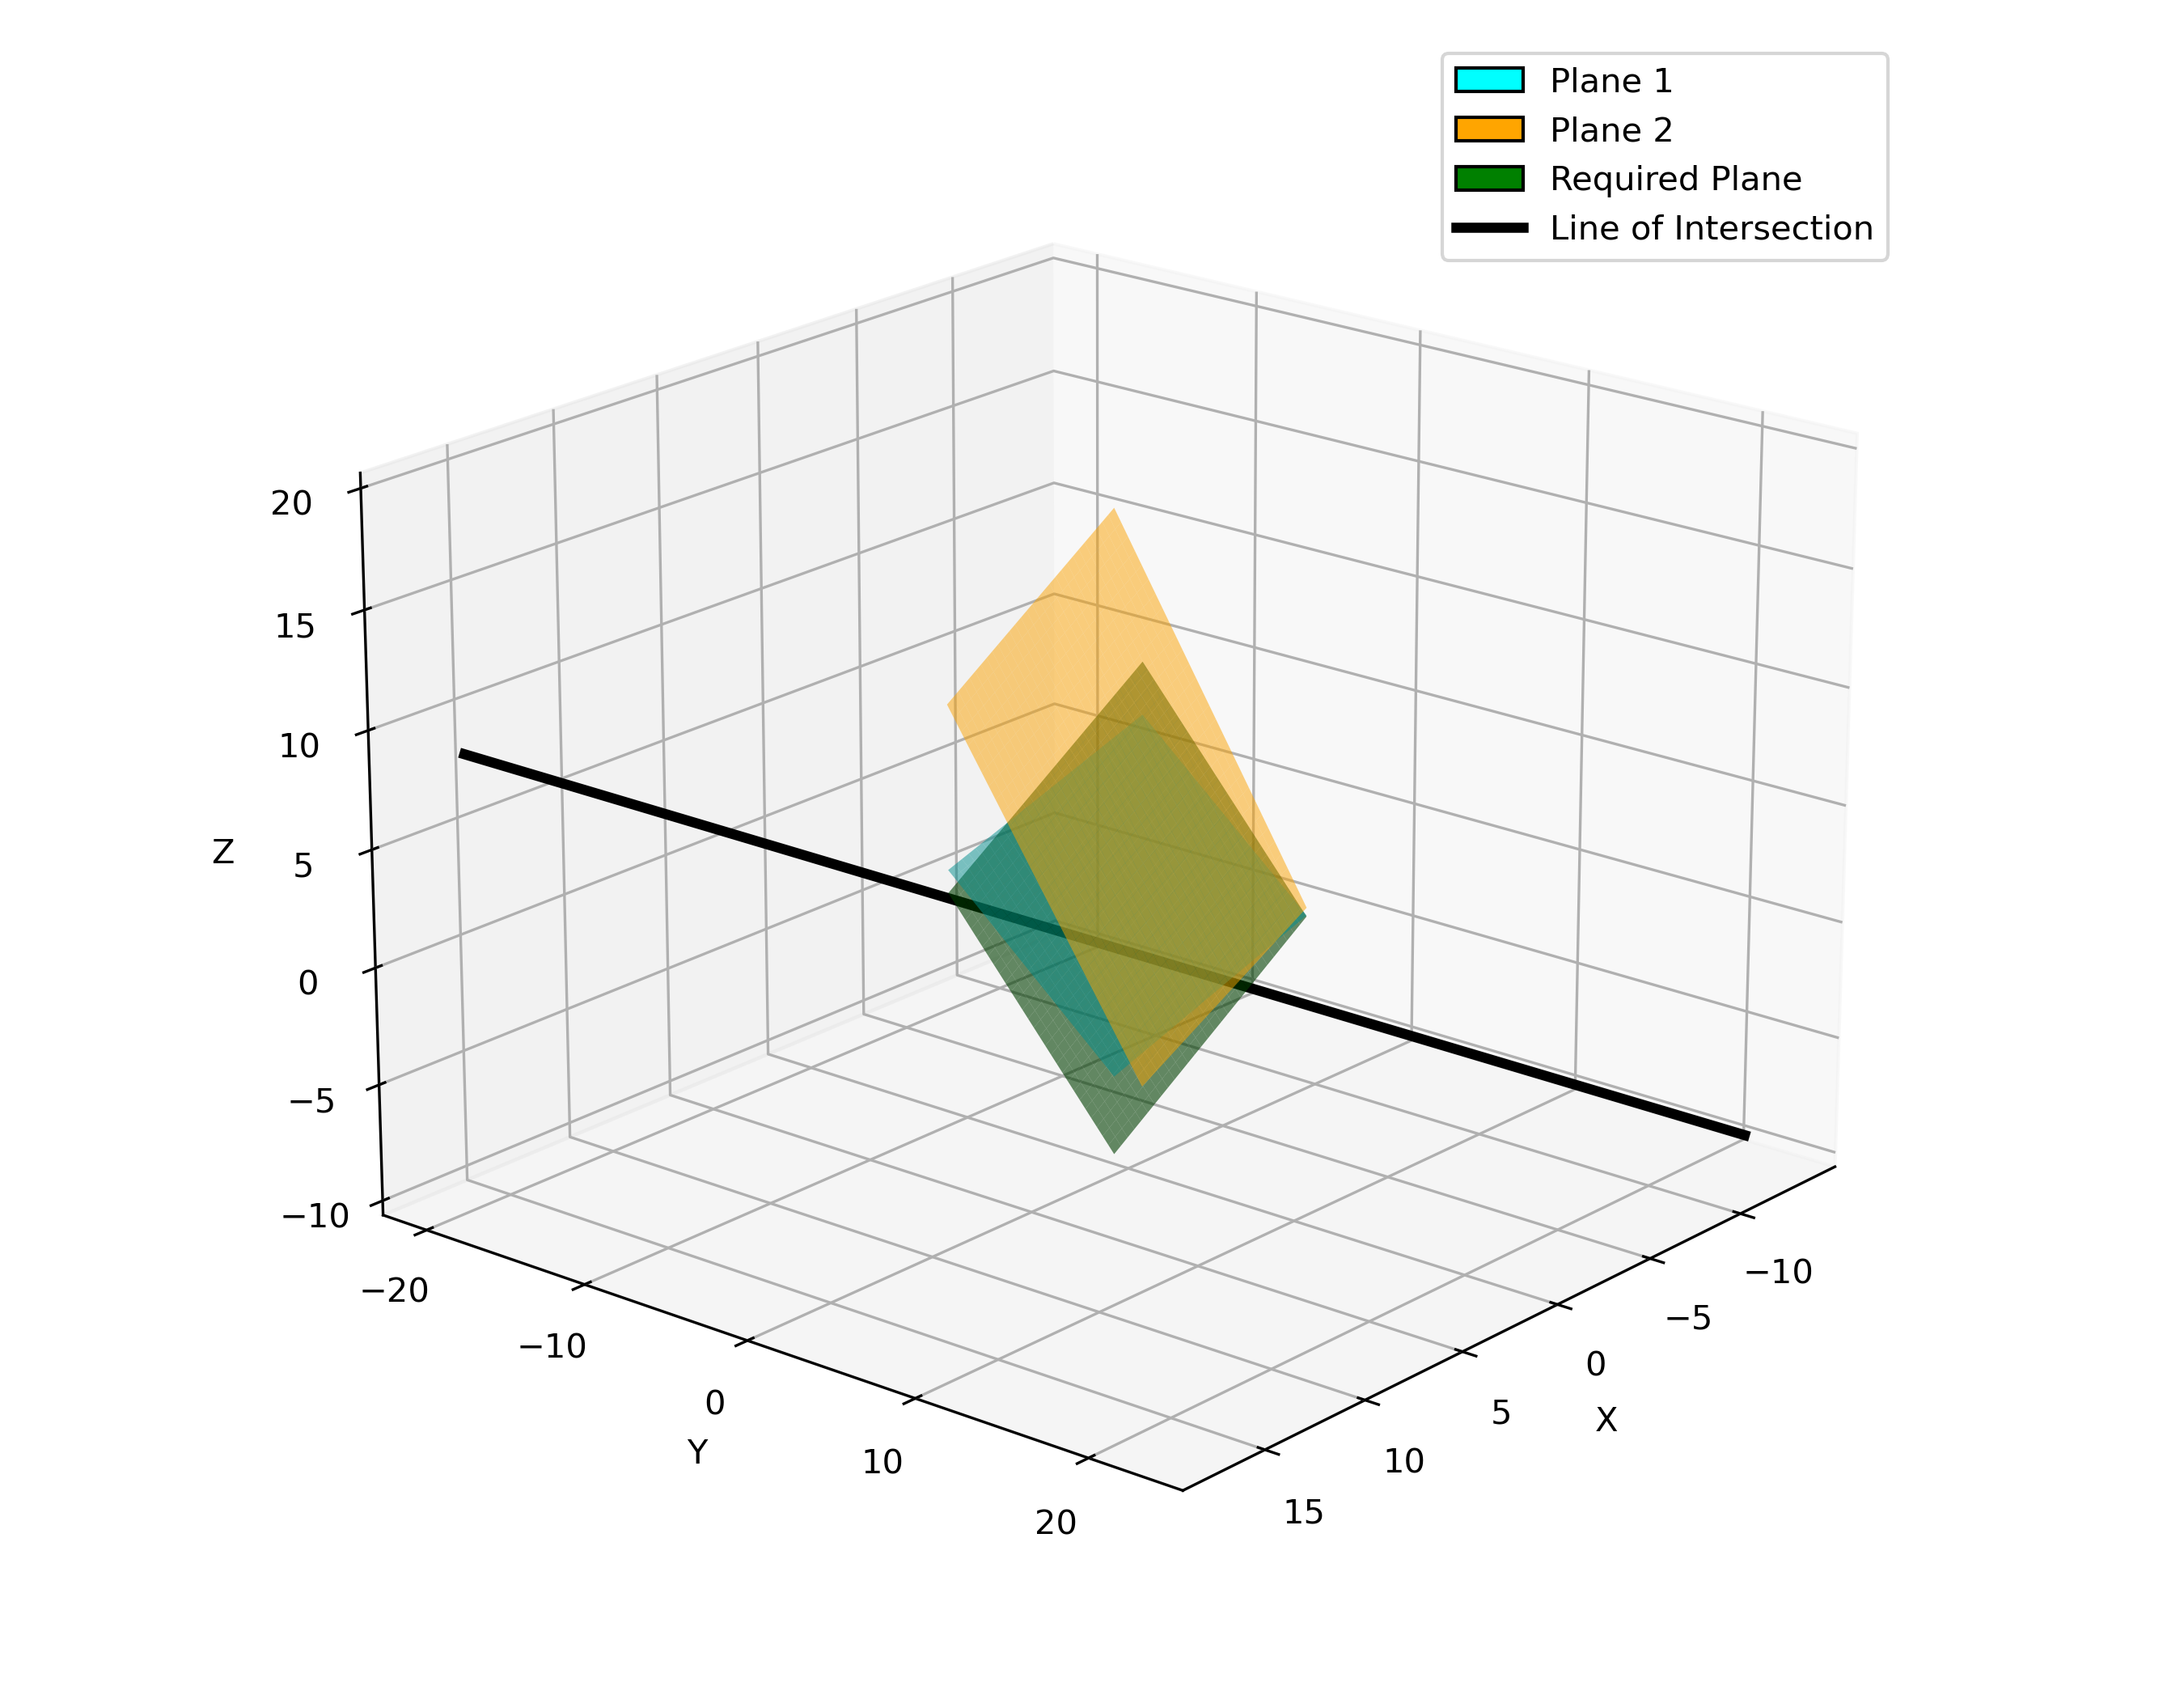
\includegraphics[width=0.9\textwidth,keepaspectratio]{figs/Figure_1.png}
\end{frame}

\end{document}
